%!TEX root = Manuscript.tex

\chapter{Precise matching}
\label{chap:intro}
\minitoc

\section{Introduction}
\subsection{Motivation}
\subsection{Contribution}
check SIFT scale and rotation\\
\textit{one-to-one tiling scheme}\\
3D ransac?

\section{Methodology}

\begin{figure*}[htbp]
	\begin{center}
		\subfigure[Workflow]{
			\begin{minipage}[t]{1\linewidth}
				\centering
				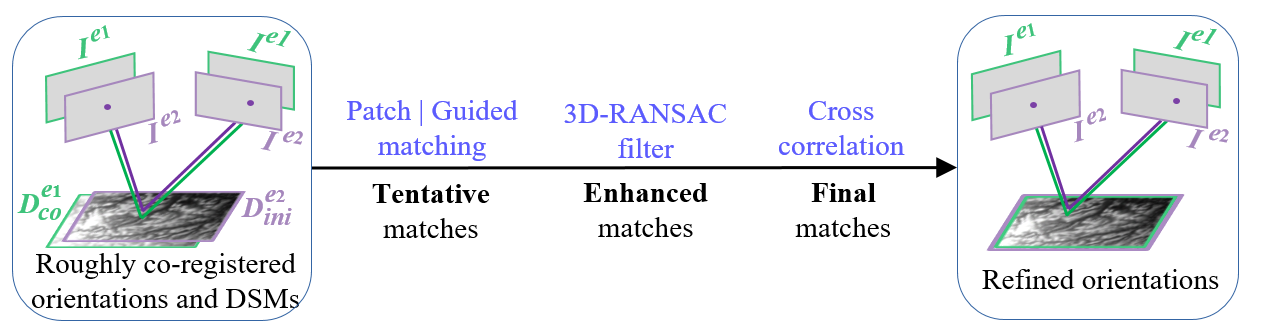
\includegraphics[width=1\columnwidth]{images/Chapitre4/precisematching.png}
			\end{minipage}%
		}
		\subfigure[Patch matching]{
			\begin{minipage}[t]{0.35\linewidth}
				\centering
				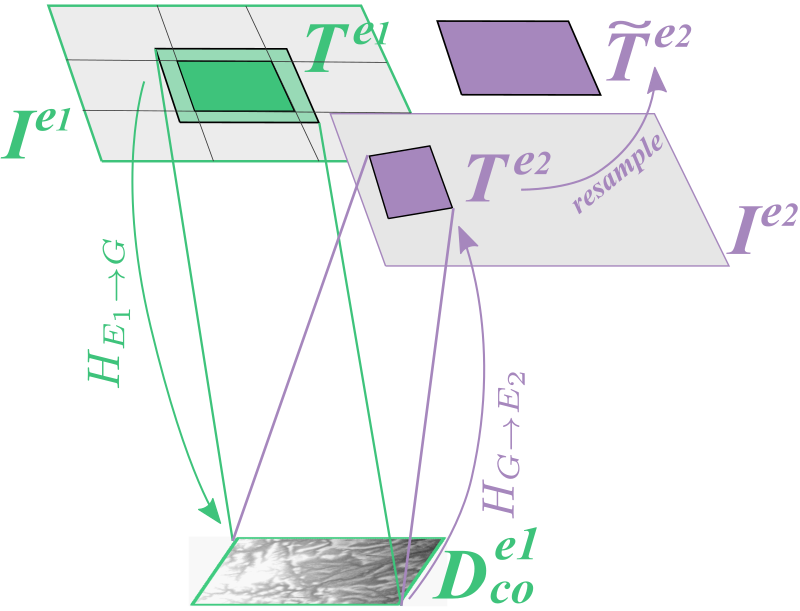
\includegraphics[width=4.5cm]{images/Chapitre4/patchmatching.png}
			\end{minipage}%
		}
		\subfigure[Buffer zone of tiles]{
	\begin{minipage}[t]{0.25\linewidth}
		\centering
		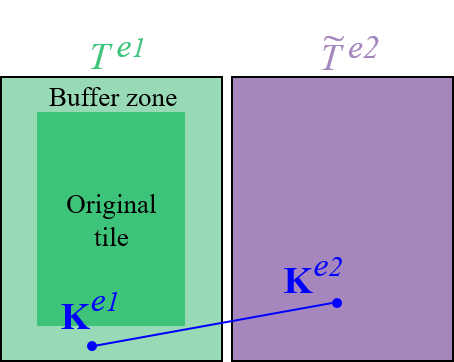
\includegraphics[width=3cm]{images/Chapitre4/tilingScheme.png}
	\end{minipage}%
}
		\subfigure[Guided matching]{
	\begin{minipage}[t]{0.35\linewidth}
		\centering
		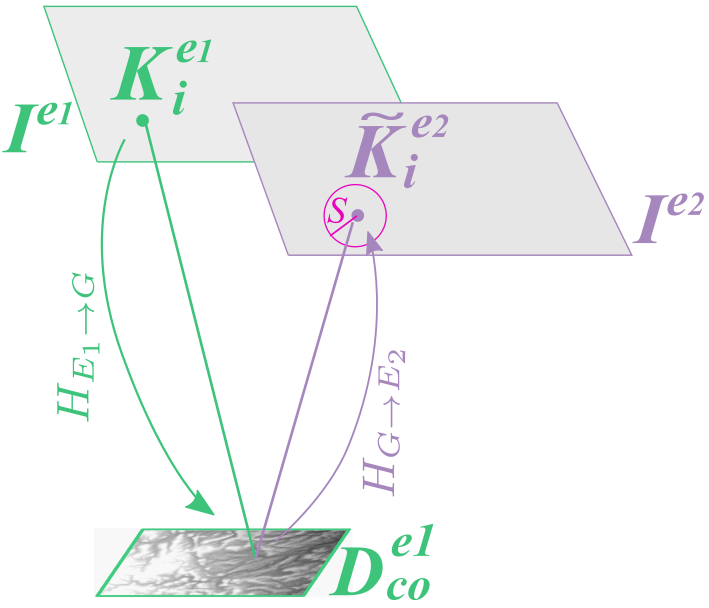
\includegraphics[width=4.5cm]{images/Chapitre4/guidedmatching.png}
	\end{minipage}%
}
		\caption{(a) Workflow of precise matching. (b) and (d)   illustrate toy-examples of the patch matching and guided matching, respectively, (c) displays the feature correspondences where $\mathbf{K}^{e_1}$ exceeds the original tile size (dark green area) and therefore will be abandoned.}
		\label{WorkflowPatch}
	\end{center}
\end{figure*}

\begin{figure*}[htbp]
	\begin{center}
			\subfigure[Example of an image pair]{
		\begin{minipage}[t]{1\linewidth}
			\centering
			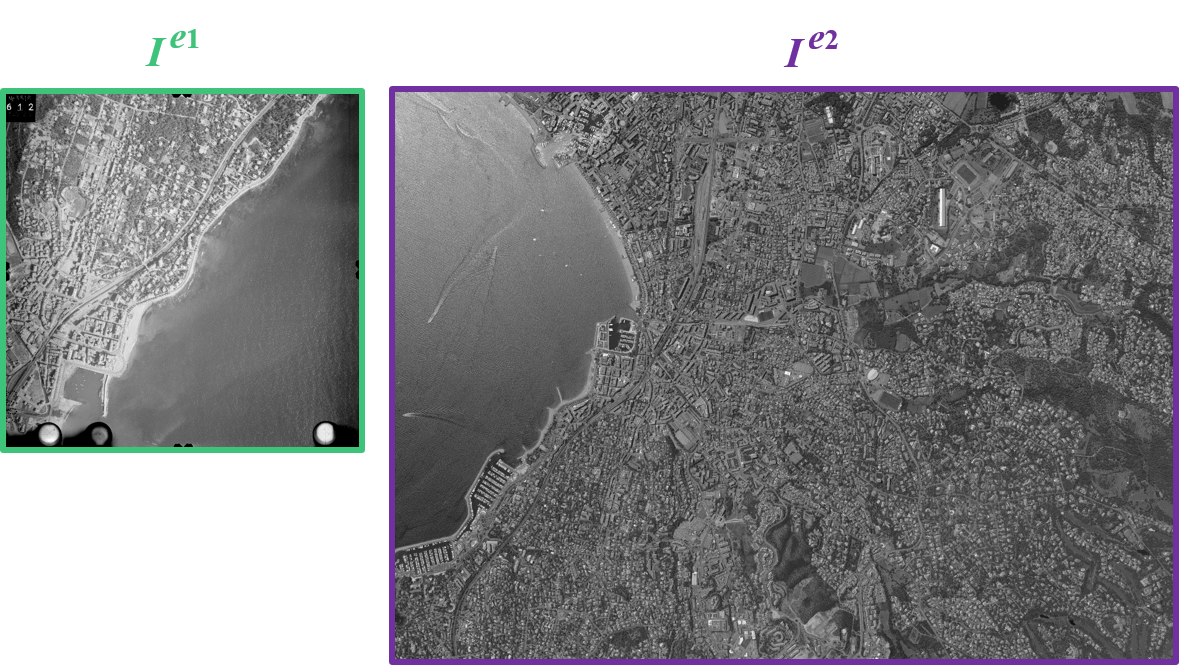
\includegraphics[width=1\columnwidth]{images/Chapitre4/example.png}
		\end{minipage}%
	}
		\subfigure[Example of patch pairs]{
			\begin{minipage}[t]{1\linewidth}
				\centering
				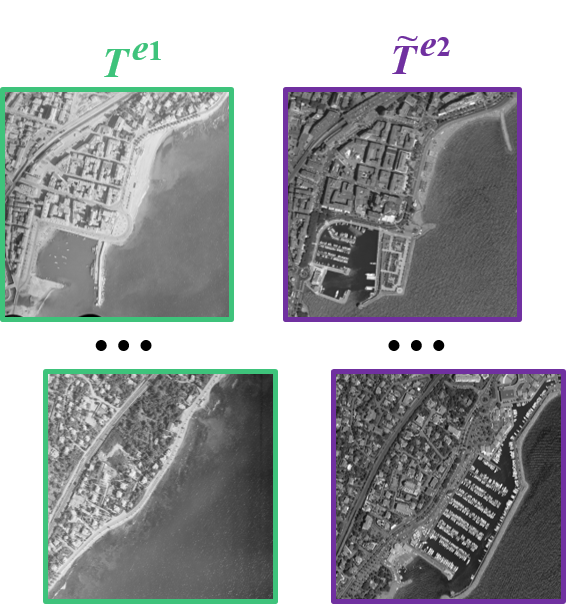
\includegraphics[width=0.5\columnwidth]{images/Chapitre4/patchexample.png}
			\end{minipage}%
		}
		\caption{(a) Example demonstration of an image pair, the master image ($I^{e_1}$) and secondary image ($I^{e_2}$) are taken at Fr{\'e}jus in 1954 and 2014 individually. (b) Patch pairs resulted from (a).}
		\label{WorkflowPatch}
	\end{center}
\end{figure*}

\begin{figure*}[htbp]
	\begin{center}
		\subfigure[Example of keypoint prediction]{
			\begin{minipage}[t]{1\linewidth}
				\centering
				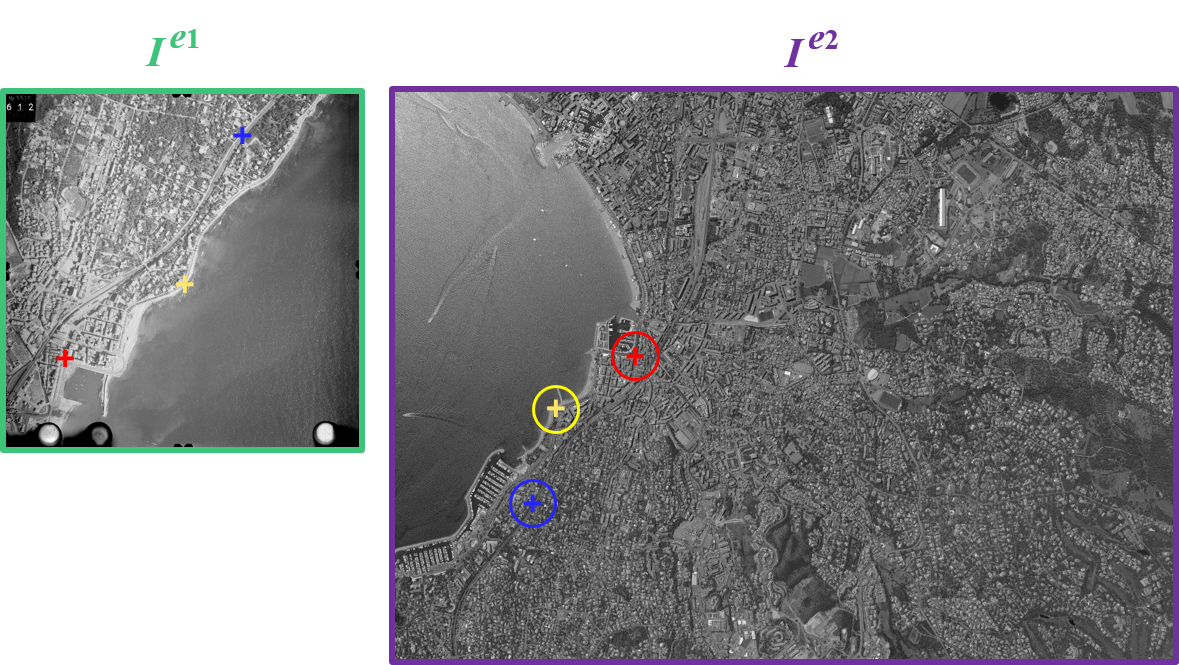
\includegraphics[width=1\columnwidth]{images/Chapitre4/guidedexample.png}
			\end{minipage}%
		}
		\caption{Example demonstration of keypoint prediction (cross symbols) accompanied with search space (circles) on an image pair, the master image ($I^{e_1}$) and secondary image ($I^{e_2}$) are taken at Fr{\'e}jus in 1954 and 2014 individually.}
		\label{WorkflowPatch}
	\end{center}
\end{figure*}



\section{Experiments}

\section{Conclusion}

\section{Discussion}
